\documentclass[11pt,a4paper]{article}
\usepackage[a4paper,hmargin=1in,vmargin=1in]{geometry}
\usepackage{pgfplots}
\pgfplotsset{compat=1.17}

\usepackage[british]{babel}
\usepackage[utf8]{inputenc}
\usepackage[T1]{fontenc}

\usepackage[nodayofweek]{datetime}
\newdate{Date}{18}{1}{2024}

\usepackage{stddoc}
\usepackage{subcaption}


\begin{document}

    \pagenumbering{arabic}

    % Header
    \begin{center}
        {\LARGE\textbf{B2M17NKA - Project III}}\\[3mm]
        \begin{minipage}{0.4\textwidth}
            \begin{flushleft}
                \textsc{\displaydate{Date}}
            \end{flushleft}
        \end{minipage}
        ~
        \begin{minipage}{0.4\textwidth}
            \begin{flushright}
                \textsc{Martin Šimák}
            \end{flushright}
        \end{minipage}
        \noindent\rule{14.5cm}{0.4pt}
    \end{center}

    \paragraph{Task} \emph{Design of a patch antenna with circular polarization}
    \begin{enumerate}[label=\arabic*.]
        \item Design a patch antenna with RHCP (Right-Handed Circular Polarization) for a frequency band around the resonant frequency $f_{\mathrm{res}} = 2.45\, \mathrm{GHz}$, in an electromagnetic simulator. Pattern of the patch can be chosen from the variants illustrated in Figure~\ref{fig:antenna-patterns}. The antenna is to be designed so that the reflection coefficient in resonance $\Gamma(f_{\mathrm{res}}| < -10\, \mathrm{dB}$ and the axial ratio in the perpendicular direction is smaller than $3\, \mathrm{dB}$.
        \begin{figure}[!ht]
            \centering
            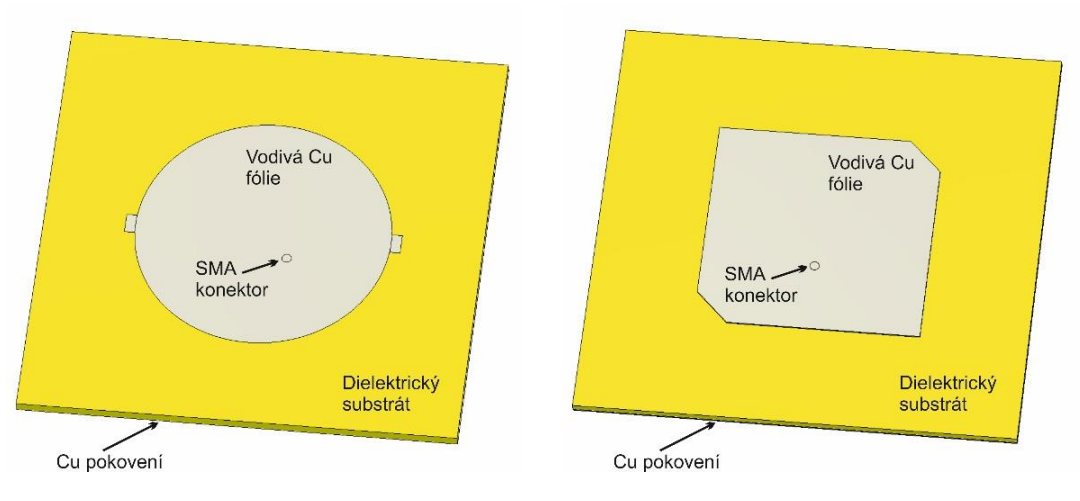
\includegraphics[width=.7\textwidth]{src/antenna-patterns.png}
            \caption{\label{fig:antenna-patterns}Possible antenna patterns}
        \end{figure}

        \item Fabricate the antenna with the help of the department. The ground plate will be the dielectric substrate FR4 ($\epsilon_r = 4.7$, $\tan(\delta) = 0.02$) of dimensions $80 \times 80 \times 1.55\, \mathrm{mm}$, with one-sided copper cladding. The antenna will be fed by a standard SMA connector (outer/inner pin diameters $4.09/1.28\, \mathrm{mm}$) filled with Teflon (PTFE). The conductive pattern will be cut out of a thin (thickness $35\, \mathrm{\mu m}$) copper foil using a plotter. This adhesive foil will be contacted directly onto the ground plate. Pay special attention to practical feasibility during the design.

        \item Measure the reflection from the fabricated antenna in the operating frequency band.
        
        \item Plot the important antenna parameters:
        \begin{enumerate}[label=4.\arabic*]
            \item reflection coefficient (simulated and measured),
            \item input impedance (simulated and measured),
            \item axial ratio angle dependence,
            \item axial ratio frequency dependence,
            \item 3D radiation pattern (simulated) and cuts in the $E$- and $H$-plane (simulated and measured).
        \end{enumerate}
    \end{enumerate}

\newpage
    \section{Antenna model}
        The antenna was designed in CST Studio Suite in accordance with the assignment. The final model is shown in Figure~\ref{fig:model}.
        \begin{figure}[!ht]
            \centering
            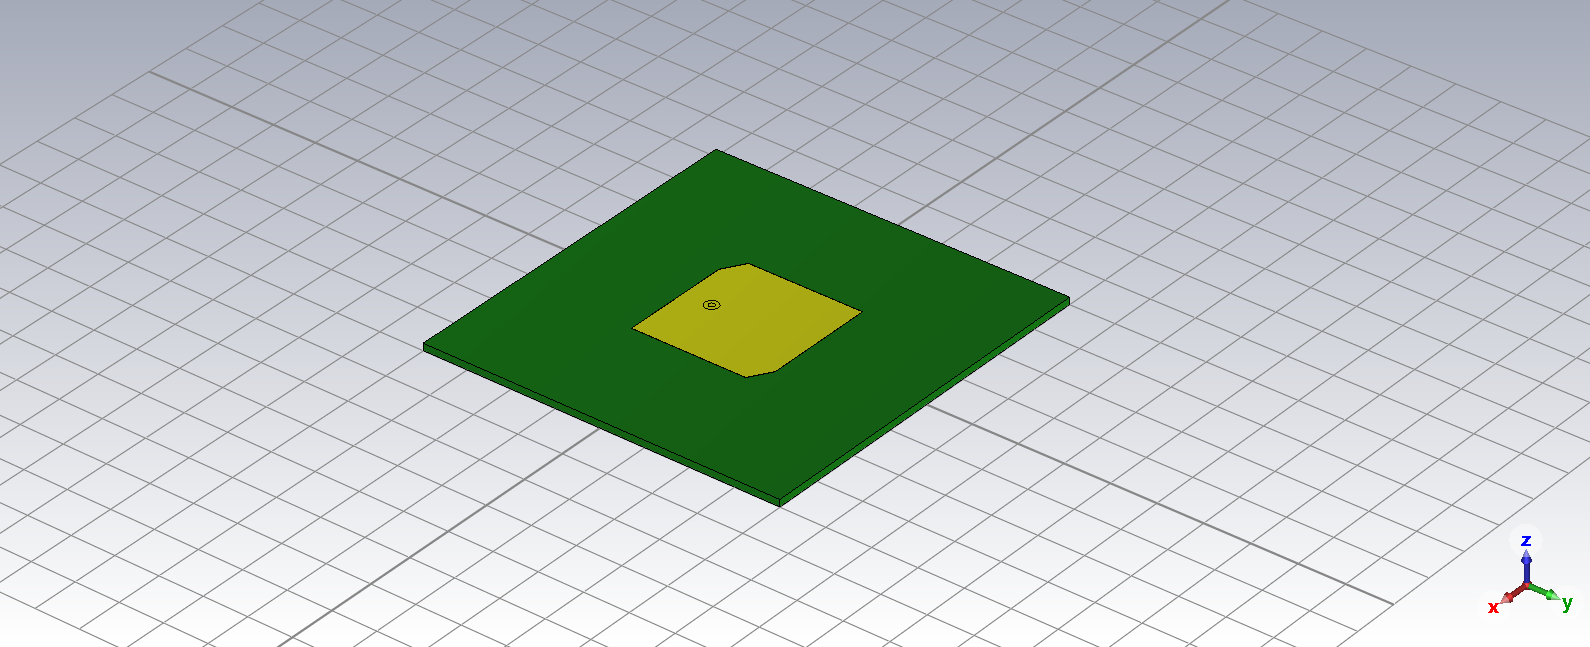
\includegraphics[width=.8\textwidth]{src/model.png}
            \caption{\label{fig:model}Antenna model}
        \end{figure}

    \section{Antenna fabrication}
        The antenna has been successfully fabricated in one of the laboratory seminars during the semester.

    \section{Fabricated antenna reflection measurement}
        The input impedance of the fabricated antenna was determined from the S-parameters (reflection coefficient) measured using a VNA.
        
    \section{Important antenna parameters}
        The antenna was both designed and fabricated to the fulfilment of the assignment. This can be seen in Figure~\ref{fig:reflection-coefficient} where the magnitude of the reflection coefficient clearly reaches the expected values around the resonant frequency. Furthermore, the input impedance is plotted by parts in Figure~\ref{fig:input-impedance}.

        Another important parameter, especially for circularly polarized antennas, is the \emph{axial ratio} expressing the minor axis to major axis ratio of the produced wave. The angle and frequency dependences of the axial ratio are shown in Figure~\ref{fig:axial-ratio-angle} and Figure~\ref{fig:axial-ratio} respectively.
        
        The radiation properties are conveyed both in 3D and 2D. Figure~\ref{fig:farfield} shows the 3D farfield pattern. The radiation patterns can also be inspected in cuts through the $E$- and $H$-plane in Figure~\ref{fig:radiation-patterns}.
\newpage
        \begin{figure}[!ht]
            \centering
            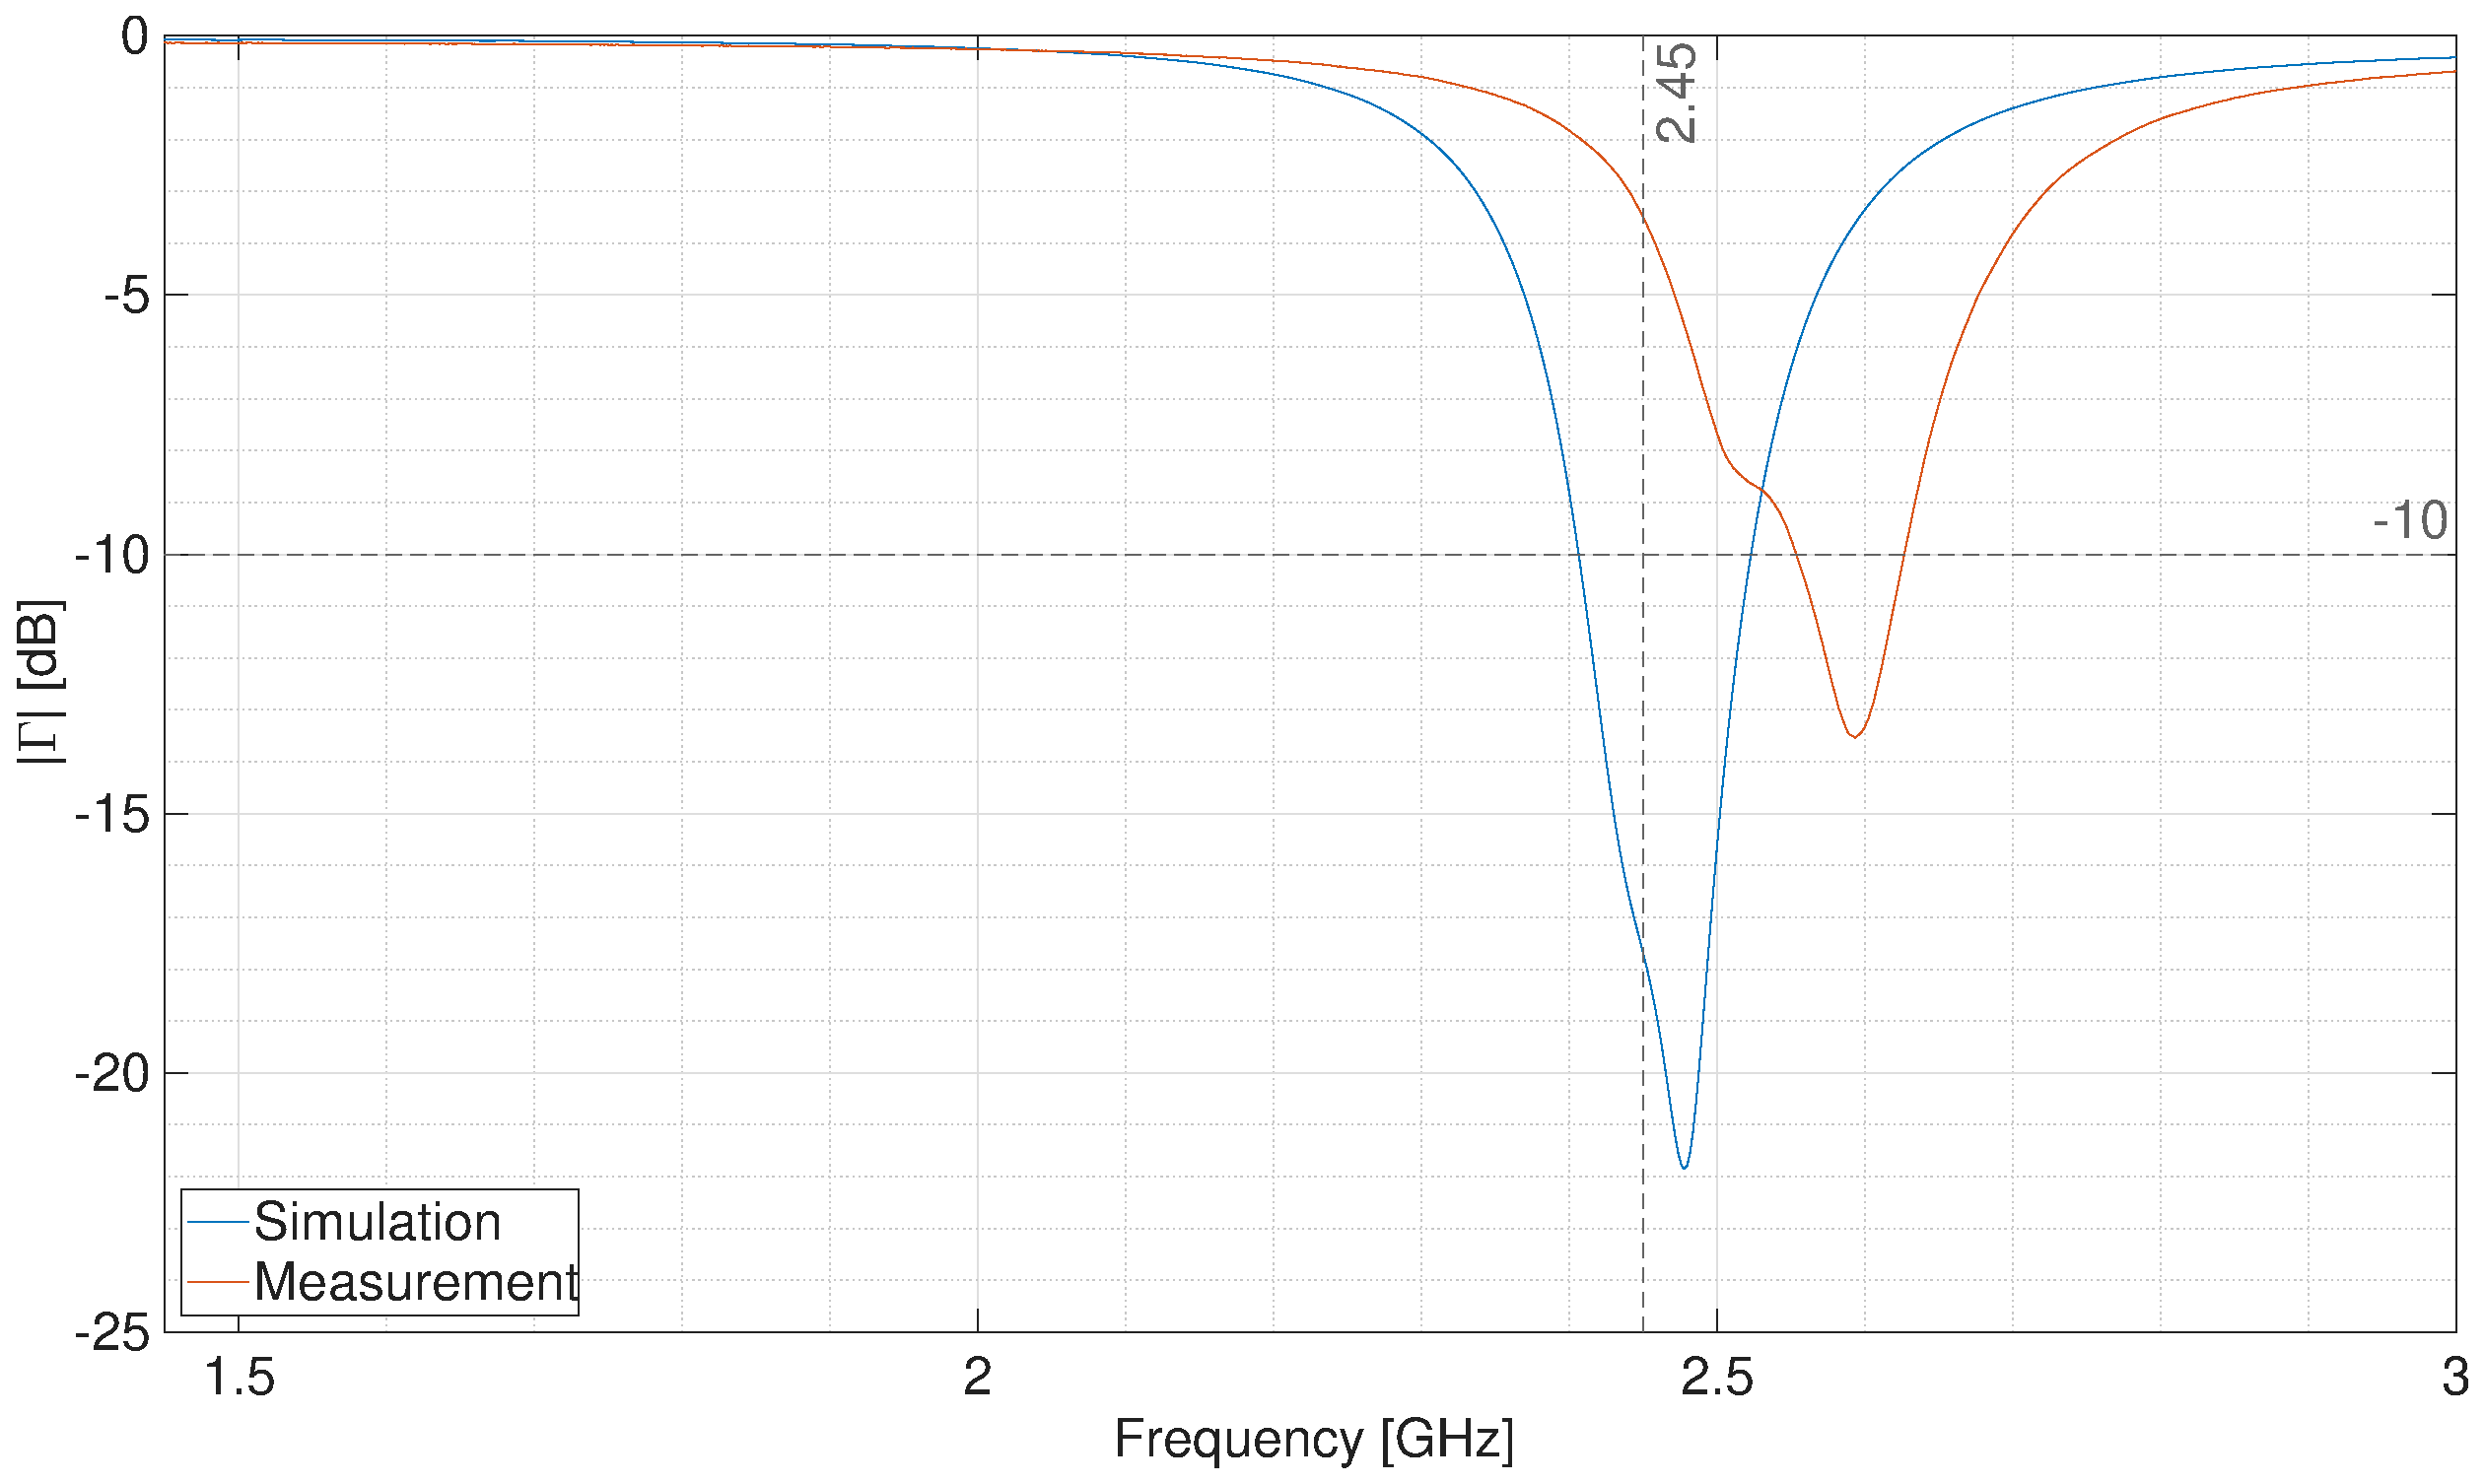
\includegraphics[width=.8\textwidth]{src/reflection-coefficient.eps}
            \caption{\label{fig:reflection-coefficient}Reflection coefficient}
        \end{figure}

        \begin{figure}[!ht]
            \centering
            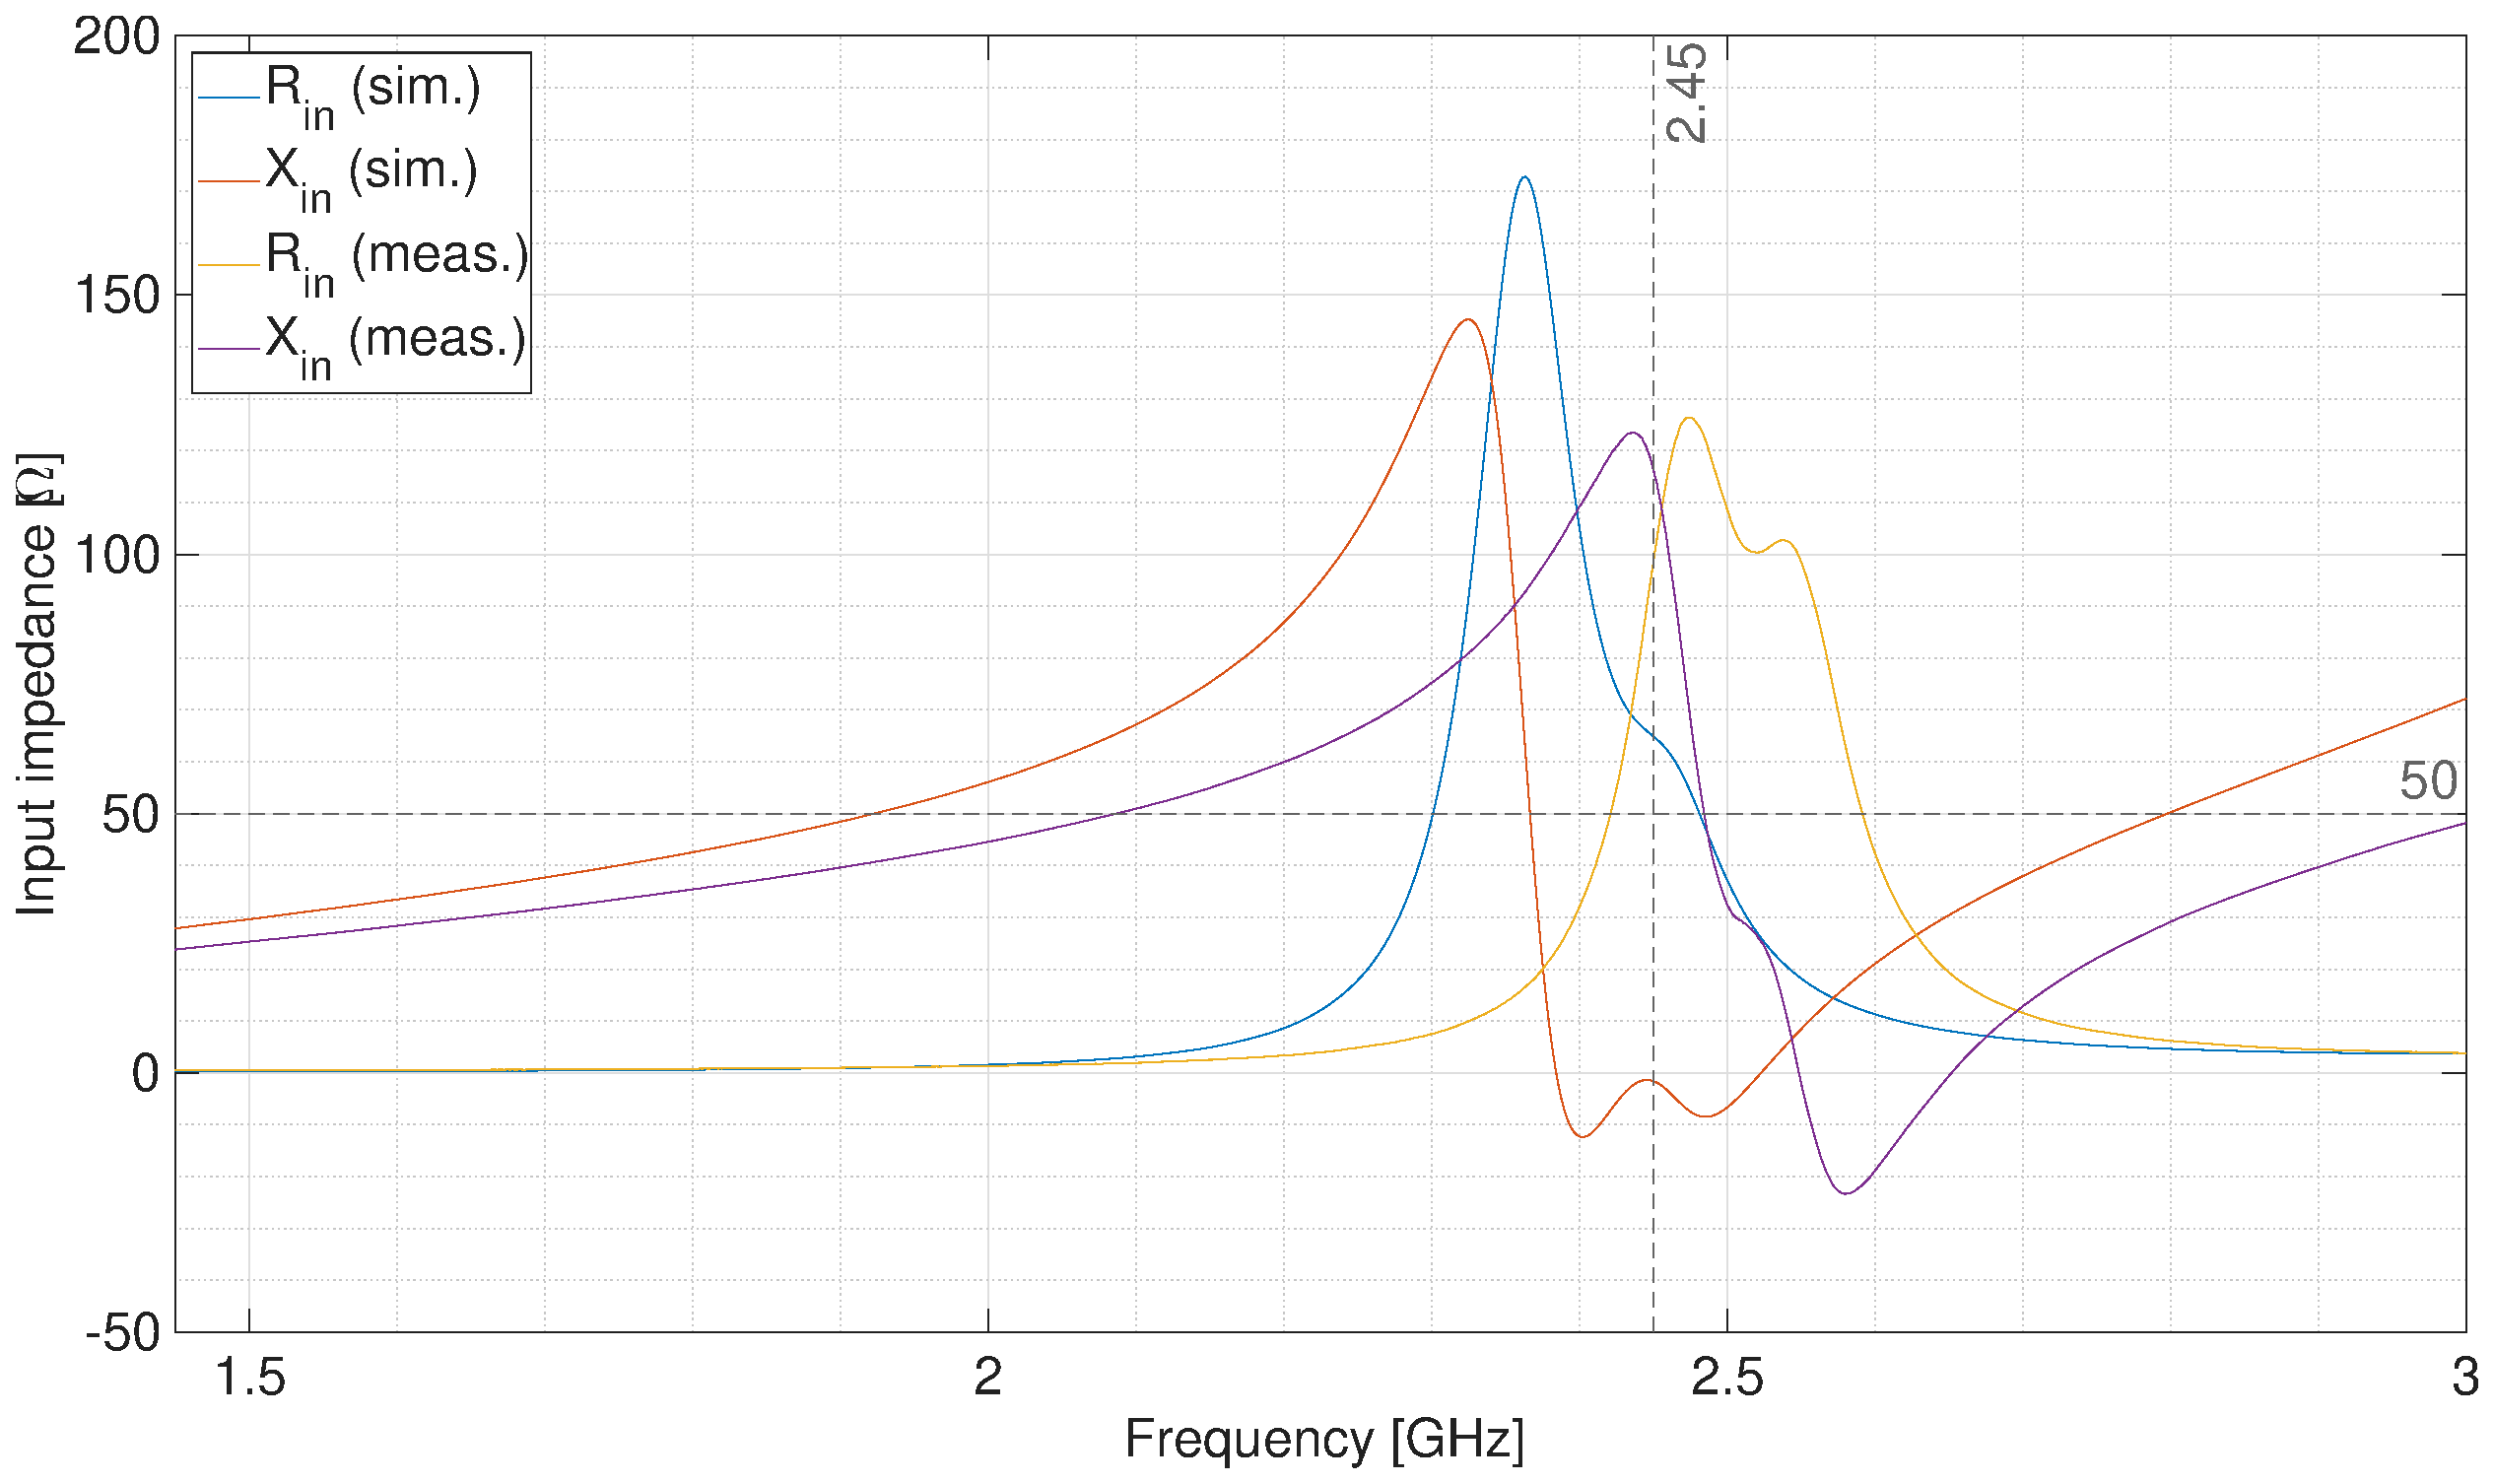
\includegraphics[width=.8\textwidth]{src/input-impedance.eps}
            \caption{\label{fig:input-impedance}Input impedance}
        \end{figure}

        \begin{figure}[!ht]
            \centering
            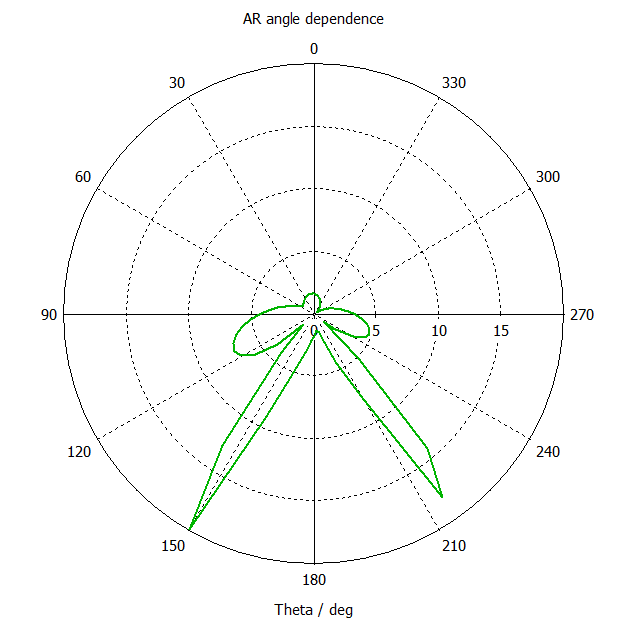
\includegraphics[width=.7\textwidth]{src/axial-ratio-angle.png}
            \caption{\label{fig:axial-ratio-angle}Axial ratio angle dependence ($\varphi=0$)}
        \end{figure}

        \begin{figure}[!ht]
            \centering
            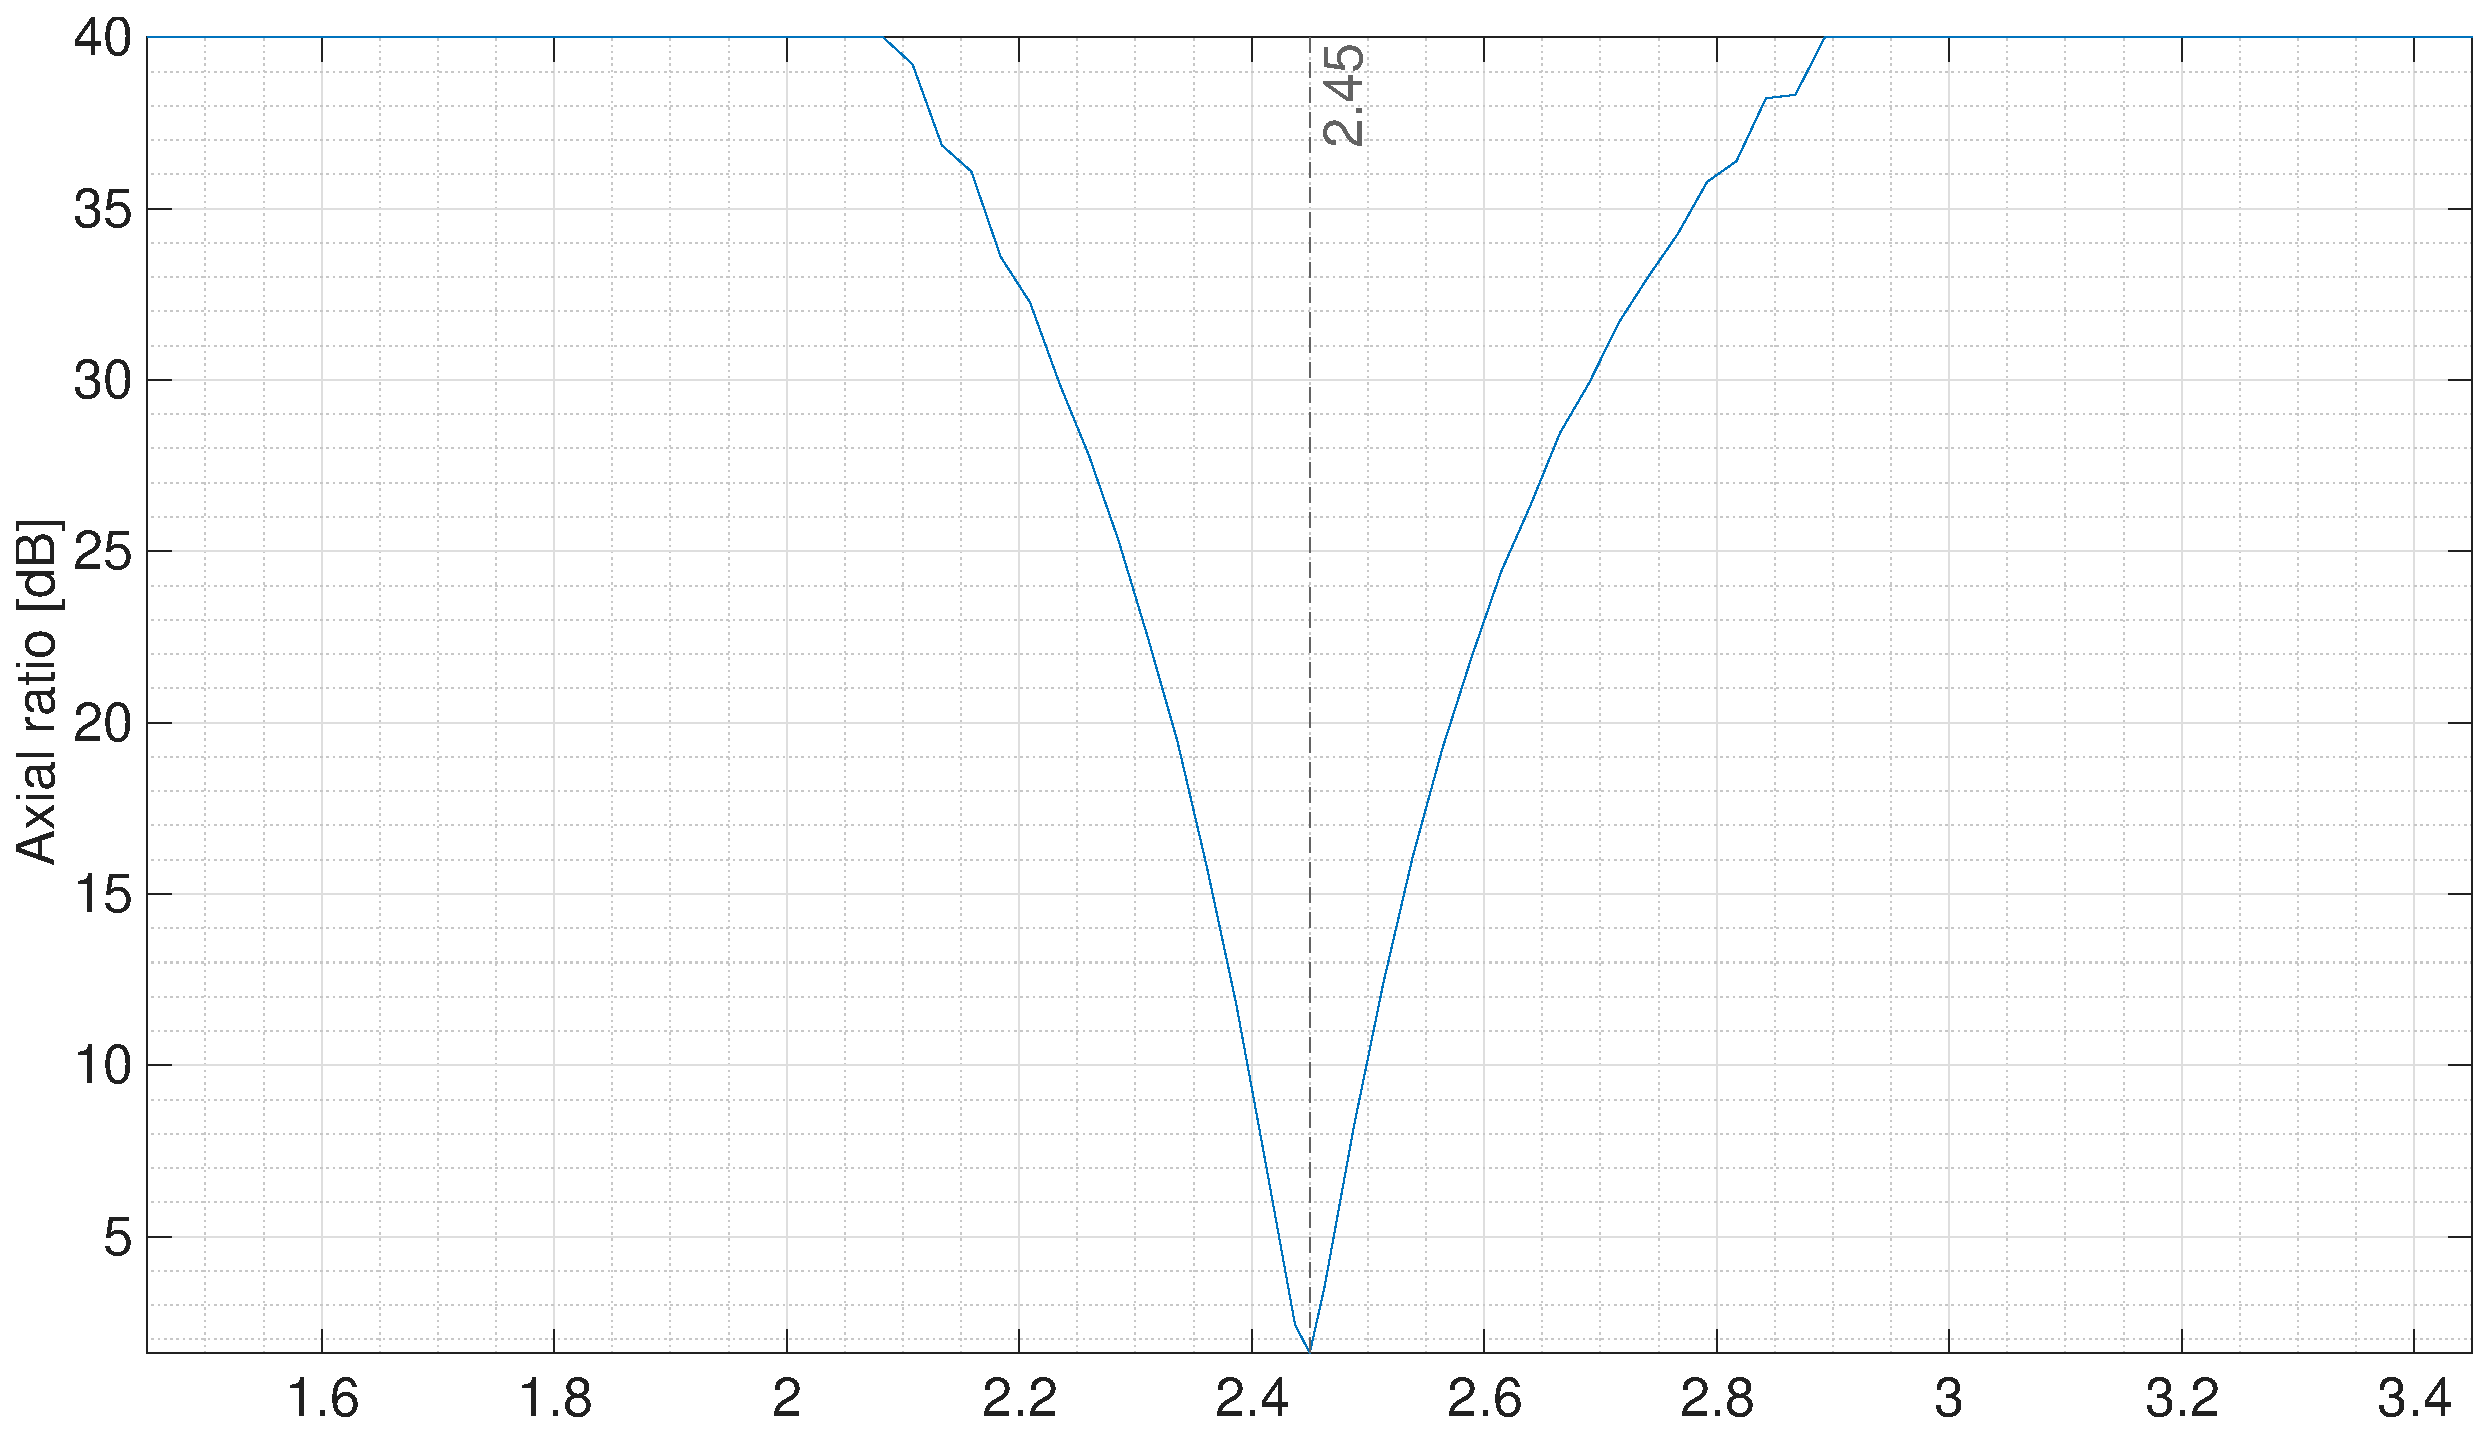
\includegraphics[width=.8\textwidth]{src/axial-ratio.eps}
            \caption{\label{fig:axial-ratio}Axial ratio frequency dependence}
        \end{figure}

        \begin{figure}[!ht]
            \centering
            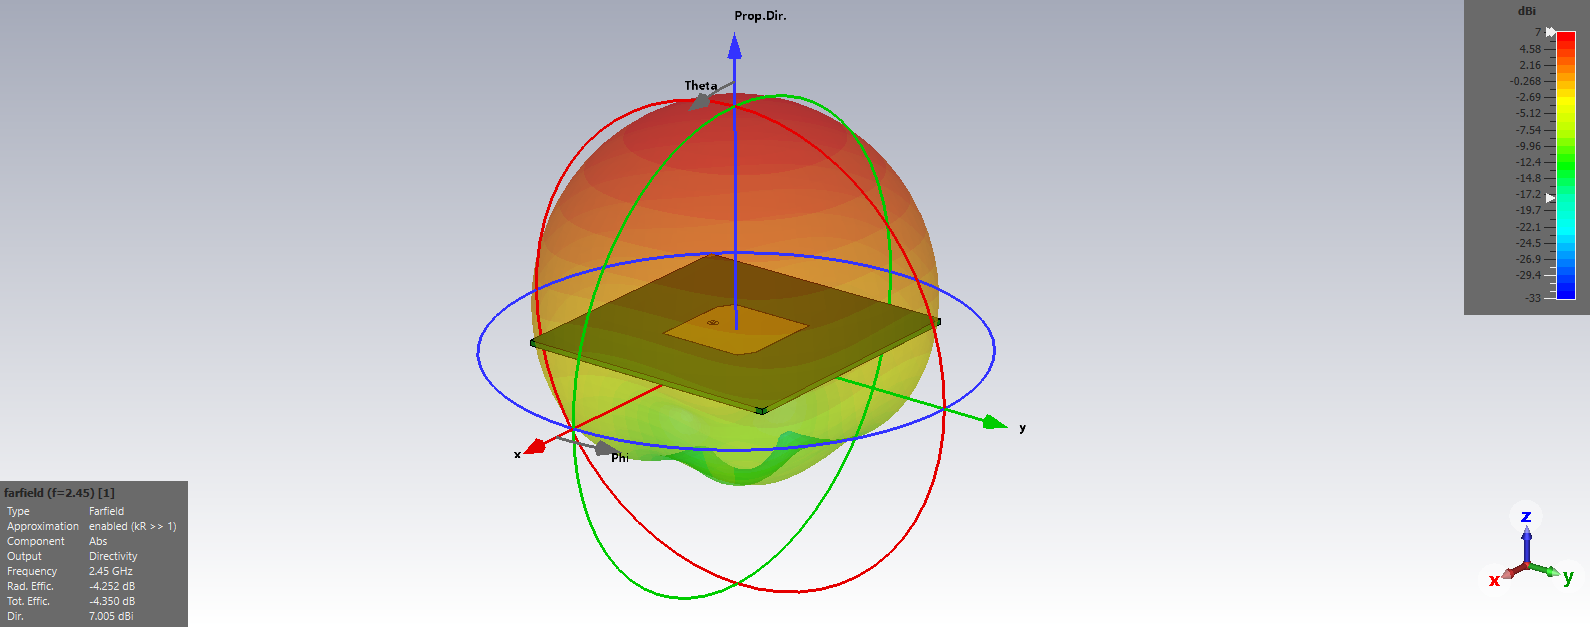
\includegraphics[width=.8\textwidth]{src/farfield.png}
            \caption{\label{fig:farfield}3D farfield pattern}
        \end{figure}

        \begin{figure}[!ht]
            \centering
            \begin{subfigure}{.4\textwidth}
                \centering
                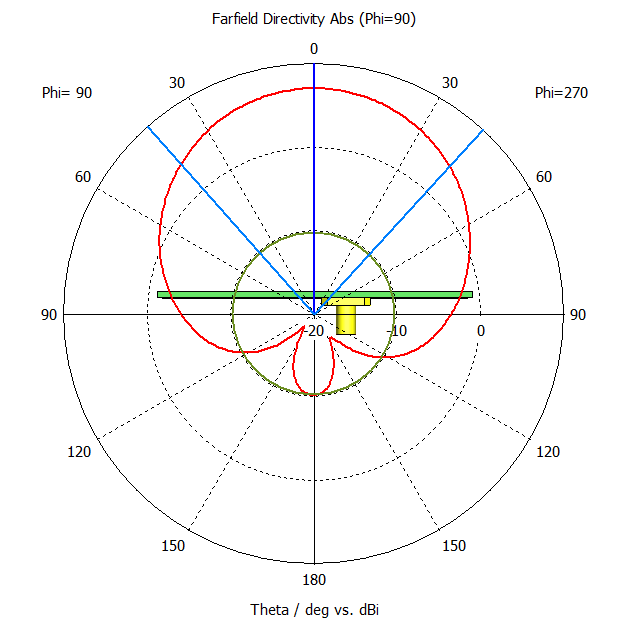
\includegraphics[width=\textwidth]{src/radiation-e.png}
                \caption{\label{fig:radiation-e}$E$-plane}
            \end{subfigure}
            ~
            \begin{subfigure}{.4\textwidth}
                \centering
                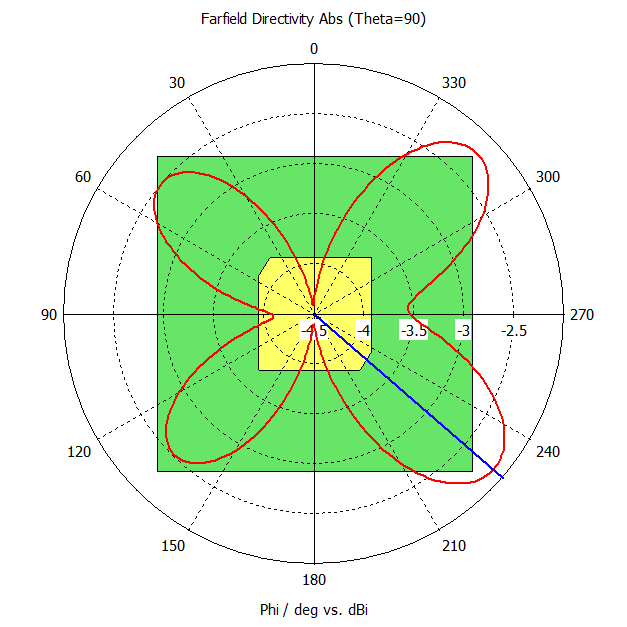
\includegraphics[width=\textwidth]{src/radiation-h.png}
                \caption{\label{fig:radiation-h}$H$-plane}
            \end{subfigure}
            \caption{\label{fig:radiation-patterns}Radiation patterns}
        \end{figure}
        

\end{document}
